\newcommand{\uco}{\fun{uco}}
\newcommand{\lfp}{\fun{lfp}}
\newcommand{\wide}{\nabla}

\chapter{Teoria dei reticoli}\label{chap:teoriareticoli}

\section{Poset}

\begin{definition}[Poset]
Un \emph{insieme parzialmente ordinato} o \emph{poset} è una struttura $\struct{P, \sqsubseteq}$ tale che $P$ è un insieme e $\sqsubseteq$ è una relazione binaria su $P$ che gode di proprietà \emph{riflessiva}, \emph{antisimmetrica} e \emph{transitiva}. 
\end{definition}

In una relazione d'ordine parziale $\sqsubseteq$ non è detto che tra due elementi $x,y \in P$ questi siano confrontabili, cioè che valga $x \sqsubseteq y \lor y \sqsubseteq x$. In questo caso si scrive $x || y$. Se tutti gli elementi dell'insieme sono a due a due confrontabili, la relazione d'ordine si dice \emph{totale} e viene indicata col simbolo $\le$. 

Esempi di poset le strutture $\struct{\mathbb{Z}, \le}$ (che è anche un insieme totalmente ordinato), la struttura $\struct{\wp(S), \subseteq}$ formata dall'insieme delle parti di un insieme $S$ e la relazione di inclusione insiemistica (Figura~\ref{fig:poset-parti}), ma anche la struttura $\struct{\{1,2,3,4,6,12\}, \mathbf{divide}}$.

\begin{figure}[htbp]
    \centering
    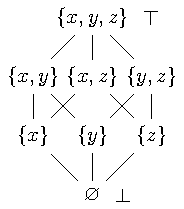
\includegraphics{appendici/immagini/poset-parti.pdf}
    \caption{Poset $\struct{\wp(S), \subseteq}$ con $S = \{x,y,z\}$}
    \label{fig:poset-parti}
\end{figure}

\begin{definition}[Elementi top e bottom]
All'interno di un poset $\struct{P, \sqsubseteq}$ si può individuare, se esiste, l'elemento top $\top \in P$ tale che $\forall x \in P . x \le \top$. Se l'elemento $\top$ esiste, è unico. L'elemento bottom $\bot$ è definito in modo duale.
\end{definition}

All'interno del poset $\struct{\wp(S), \subseteq}$ l'elemento top è $\top = S$ e il bottom è $\bot = \varnothing$. All'interno del poset $\struct{\mathbb{Z}, \le}$ non esiste l'elemento top ma esiste l'elemento bottom $\bot = 0$. Se ad $\mathbb{Z}$ aggiungiamo un ulteriore elemento $\infty$ tale che $\forall n \in \mathbb{Z} . n < \infty$ allora questo elemento funge da top per la nuova struttura $\struct{\mathbb{Z} \cup \{ \infty \}, \le}$ creata.

\begin{definition}[Least upper bound]
L'operazione di \emph{least upper bound} (o \emph{lub}, \emph{join}, \emph{estremo superiore}) tra due elementi $x,y \in P$ di un poset $\struct{P, \sqsubseteq}$ se esiste è l'elemento $\join[x][y] = z \in P$ tale che:
\begin{itemize}
    \item $\join[x][y]$ è maggiorante di $x$ e $y$ ($x,y \sqsubseteq \join[x][y]$);
    \item $\join[x][y]$ è il più piccolo maggiorante di $x$ e $y$ ($\forall m \in P . (x,y \sqsubseteq m \to \join[x][y] \sqsubseteq m)$);
    \item $\join[x][y]$ è unico.
\end{itemize}
\end{definition}

\begin{definition}[Greatest lower bound]
L'operazione di \emph{greatest lower bound} (o \emph{glb}, \emph{meet}, \emph{estremo inferiore}) è definito in modo duale al lub e di indica con $\meet[x][y]$ per $x,y \in P$.
\end{definition}

Il join (e il meet) di due elementi del poset può non essere definito per due motivi: \emph{l'elemento manca} (in $\struct{\{1,2,3,4,6,12,13\}, \mathbf{divide}}$ l'elemento $\join[12][13]$ non è definito poichè non c'è elemento maggiorante di entrambi) oppure \emph{non è rispettata la condizione di unicità} (se ci sono più maggioranti non confrontabili tra loro).

\begin{definition}[Catena]
Un sottoinsieme $C \subseteq P$ del poset $\struct{P, \sqsubseteq}$ è detto \emph{catena} se gli elementi di $C$ sono a due a due confrontabili tra loro. Il duale della catena è l'anticatena (elementi non confrontabili tra loro).  
\end{definition}

\begin{definition}[Condizione ACC]
Una catena $C$ soddisfa la \emph{ascending chain condition} se $C$ è un insieme finito oppure se da un certo $n$ in poi si ha $\forall m > n . c_n = c_m$.
\end{definition}

\begin{definition}[Poset completo]
Un poset $\struct{P, \sqsubseteq}$ si dice completo (abbreviato \emph{c.p.o.}) se per ogni sua catena $C$ anche infinita esiste l'estremo superiore $\join[C] \in P$.
\end{definition}

\subsection{Reticoli}

\begin{definition}[Reticolo]
Un reticolo è una struttura $\struct{P, \sqsubseteq, \join, \meet}$ nella quale $\struct{P, \sqsubseteq}$ è un poset, l'operazione binaria $\join$ effettua il lub, l'operazione $\meet$ effettua il glb ed 
\[ \forall x,y \in P \text{ sono definiti } \join[x][y], \meet[x][y] \in P \]
\end{definition}

\begin{definition}[Sottoreticolo]
Un sottoinsieme $Q \subseteq P$ del reticolo $\struct{P, \sqsubseteq, \join, \meet}$ è detto \emph{sottoreticolo} se $Q$ è chiuso per lub e glb ($\forall x,y \in Q . \join[x][y], \meet[x][y] \in Q$). 
\end{definition}

\begin{definition}[Reticolo completo]
Un reticolo che è anche c.p.o. viene detto reticolo completo.
\end{definition}

\subsection{Connessione di Galois}\label{sec:galois}

La definizione di connessione di Galois e inserzione di Galois si trovano rispettivamente alle Sezioni~\ref{sec:galois-c},~\ref{sec:galois-i}.

\begin{theorem}[Connessione di Galois come adjunctor]
La struttura è detta anche \emph{adjunctor} ($\alpha$ left adjoint, $\gamma$ right adjoint) poichè vale che
$$\forall c \in C, a \in A \; : \; \alpha(c) \preceq a \Leftrightarrow c \le \gamma(a)$$
\end{theorem}

\begin{theorem}[Connessione di Galois come funzioni additive e co-additive]
In una connessione di Galois la funzione $\alpha$ è additiva, cioè preserva l'operazione di join: 
$$\alpha\left(\join[X]\right) = \join[\alpha(X)] \text{ per ogni } X \subseteq C$$
e la funzione $\gamma$ è co-additiva, cioè preserva l'operazione di meet.
\end{theorem}

\section{Closure operators}

\begin{definition}[Upper closure operator]
Una funzione $\uco: L \to L$ è detta \emph{upper closure operator} se
\begin{enumerate}
    \item monotona: $x \le y \to \uco(x) \le \uco(y)$;
    \item estensiva: $x \le \uco(x)$;
    \item idempotente: $\uco(\uco(x)) = \uco(x)$.
\end{enumerate}
\end{definition}

\begin{definition}[Lower closure operator]
Una $\mathrm{lco}$ è la funzione definita dualmente rispetto ad $\uco$, riduttiva invece che estensiva.
\end{definition}

Il closure operator cattura l'essenza del processo di astrazione: la monotonicità assicura l'astrazione monotonica degli oggetti del dominio (cosa vuol dire dcane), l'idempotenza che il processo di approssimazione è svolto tutto in una volta, e l'estensività vuol dire che astrae, cioè contiene meno informazioni \footnote{Uniform Closures: Order-Theoretically Reconstructing Logic Program Semantics and Abstract Domain Refinements}.

\begin{definition}[Famiglia di Moore]
Dato un reticolo completo $L$ e un suo sottoinsieme $X \subseteq L$, chiamiamo $X$ \emph{Moore family} di $L$ se 
$$X = \mathcal{M}(X) = \{ \meet[S] \; | \; S \subseteq X \}$$
\end{definition}

Moore closure: least (w.r.t. inclusion) subset of C which contains X and is a moore family of C. \footnote{Making Abstract Interpretations Complete}

\begin{theorem}[Uco come insieme di fixpoint]
Ogni closure operator $\rho \in \uco(C)$ è identificato univocamente dal suo insieme di fixpoint $\rho(C)$, che è anche la sua immagine.

Vicecersa, $Y \subseteq C$ è un insieme di fixpoint di un $\uco$ se e solo se $Y$ è una moore family. In tal caso, $\rho_Y = \lambda x . \meet[\{y \in Y \; | \; x \le y\}]$
\end{theorem}

\begin{definition}[Reticolo degli uco]
Viene definito il reticolo degli $\uco$ sul reticolo completo $C$ la struttura
$$\struct{\uco(C), \sqsubseteq, \join, \meet, \lambda x . \top, \lambda x . x}$$
dove
\begin{itemize}
    \item $\uco(C)$: l'insieme degli upper closure operator su $C$;
    \item $\sqsubseteq$ relazione d'ordine: $\rho \sqsubseteq \eta 
        \Leftrightarrow \left(\forall c \in C . \rho(c) \le \eta(c) \right)
        \Leftrightarrow \left(\eta(C) \sqsubseteq \eta(C) \right)$;
    \item $\join$ join: $\left(\join[\rho_i]\right)(x) = x \Leftrightarrow \forall i . \rho(x) = x$;
    \item $\meet$ meet: $\left(\meet[\rho_i]\right)(x) = x \Leftrightarrow \meet[\rho_i(x)]$;
    \item $\lambda x . \top$: top;
    \item $\lambda x . x$: bottom;
\end{itemize}
\end{definition}

\section{Fixpoint}

\begin{definition}[Fixpoint]
Data $f:X \to X$, il punto $x \in X$ si definisce fixpoint se $f(x) = x$.
\end{definition}

\begin{definition}[Least fixed point]
Data $f:X \to X$, il punto $\lfp(f) = x \in X$ si definisce \emph{least fixed point} se per ogni $y$ fixpoint si ha $x \le y \to x = y$.
\end{definition}

\begin{theorem}[Teorema di Knaster-Tarski]
Data una funzione $f:L \to L$ monotona su un reticolo completo $\struct{L, \le}$ esiste un unico $\lfp(f)$.
\end{theorem}

E' possibile calcolare $\lfp(f)$ tramite il metodo iterativo:
$$\bot \le f(\bot) \le f^2(\bot) \le ... \le f^n(\bot) = \lfp(f) = f^{n+1}(\bot) = f^{n+2}(\bot) = ...$$

\section{Convergenza dei fixpoint}

Tramite il metodo iterativo, è lunga arrivare alla convergenza (a volte impossibile). Introduco operatori che accellerano la convergenza, e la garantiscono in un numero finito di passi.

\begin{definition}[Widening (binario)]
L'operatore di widening $\wide: P \to P$ su un poset $\struct{P, \le}$ soddisfa le seguenti condizioni:
\begin{itemize}
    \item $\forall x,y \in P \, . \, x \le (\wide[x][y]) \land y \le (\wide[x][y])$;
    \item Per ogni catena $x_0 \le x_1 \le ...$ si definisce la catena \emph{non strettamente crescente} $y_0 = x_0, ..., y^{n+1} = \wide[x][y^n]$.
\end{itemize}
\end{definition}

L'operatore di widening non è commutativo ne associativo. L'iterazione col widening si svolge come segue:
$$x^0 = \bot \qquad x^{n+1} = \begin{cases} 
    x^n,                & f(x^n) \le x^n \\ 
    \wide[x^n][f(x^n)], & f(x^n) \not\le x^n \\
\end{cases}$$

(todo esempio)

(vedi paper su slack)